\section{Összegzés}

\subsection{Felhasznált technológiák}
\begin{frame}
	\frametitle{Felhasznált technológiák}
	\begin{figure}[ht!]
		\centering
		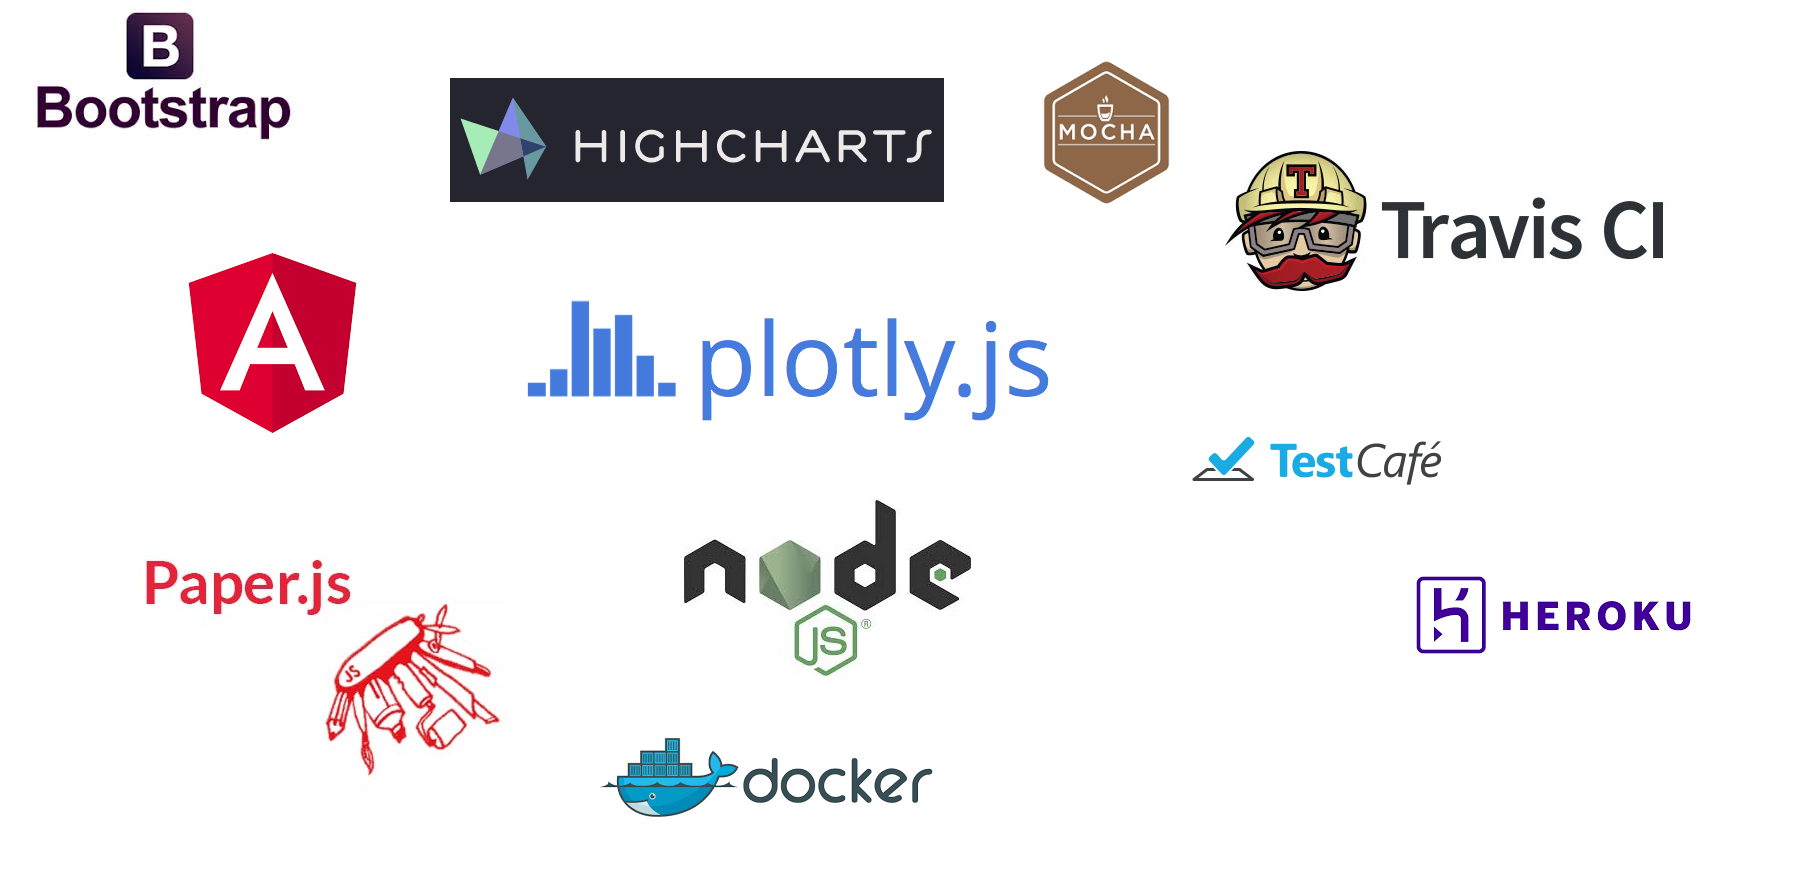
\includegraphics[width=\linewidth]{images/technologies}
	\end{figure}
\end{frame}

\begin{frame}
\frametitle{Összegzés}

\begin{block}{}
Sikerült az \cite{archetti2016cooperation} cikkbeli modellt implementálnunk valamint kiegészítenünk a sejtosztódással.
\end{block}
\begin{block}{}
A alkalmazás segítségével jobban megérthetjük, hogy mi történik egy daganaton belül
\end{block}

\pause
\begin{block}{Ez az első önálló alkalmazás, amely}
\begin{itemize}
	\item interaktívan mutatja be a sejtpopulációk változását
	\pause
	\item ezen bemutatáshoz voronoi diagramot használ
	\pause
	\item nem igényel programozási tudást, hiszen képes szimulációkat végezni pár kattintással
\end{itemize}
\end{block}
\end{frame}

\begin{frame}
\frametitle{További fejlesztési lehetőségek, célok}
\begin{itemize}
	\item további osztódási modellek tanulmányozása
	\item terápia (pl. kemoterápia) alkalmazása, ellenanyagok használata
	\item különböző ráktípusok
	\item hatékonyság növelés
	\item több típusú stratégia
\end{itemize}

\end{frame}